\subsection{Implementación}

Se completó \texttt{aStarSearch(problem, heuristic=nullHeuristic)} en \texttt{pacman/search.py}.
Reutiliza exactamente el mismo esqueleto de búsqueda en grafo que \texttt{uniformCostSearch}
(Actividad 2): misma frontera \texttt{util.PriorityQueue}, mismo diccionario \texttt{bestCost} para
no reexpandir un estado cuando ya se conoce un camino más barato, y la misma prueba de meta al
extraer el nodo de la frontera. La única diferencia es la prioridad usada para ordenar la
frontera: en UCS es $g(n)$; en A* es $f(n) = g(n) + h(n)$.

\begin{figure}[H]
\centering
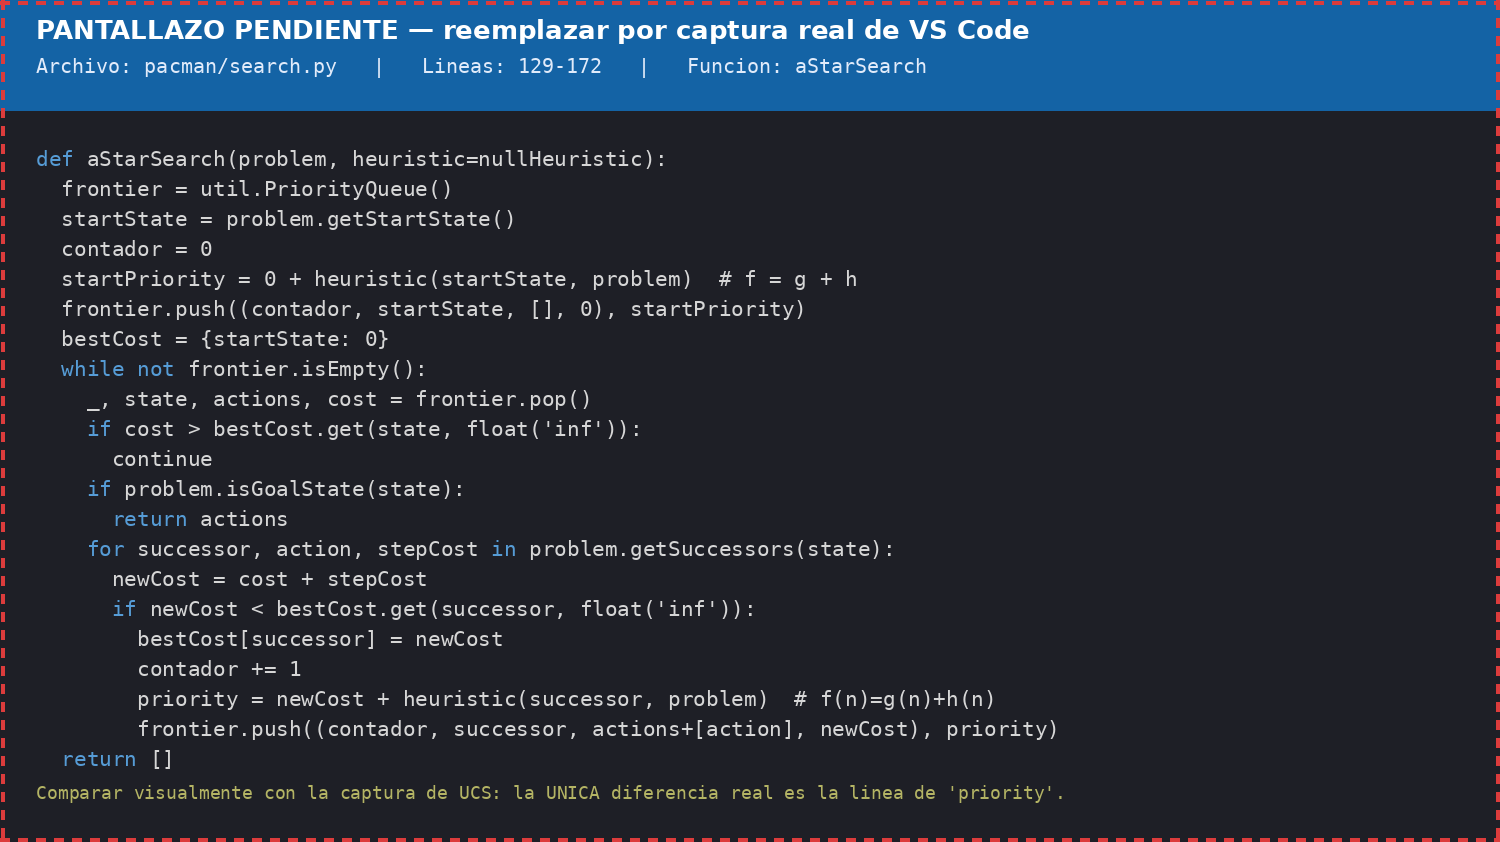
\includegraphics[width=0.95\textwidth]{capturas/actividad03_astar.png}
\caption{Implementación de \texttt{aStarSearch} en \texttt{pacman/search.py} (líneas 129-172).
Comparar con la Figura~\ref{fig:act02-ucs}: la única diferencia real es la línea de
\texttt{priority = newCost + heuristic(...)}.}
\label{fig:act03-astar}
\end{figure}

\begin{table}[H]
\centering
\caption{Los 8 requisitos de la guía y dónde se cumplen}
\label{tab:act3-requisitos}
\small
\begin{tabular}{lp{8.3cm}}
\toprule
\textbf{Requisito} & \textbf{Dónde se cumple} \\
\midrule
1. Cola de prioridad & \texttt{frontier = util.PriorityQueue()} \\
2. Comenzar desde \texttt{getStartState()} & \texttt{startState = problem.getStartState()} \\
3. Usar \texttt{isGoalState()} & \texttt{if problem.isGoalState(state): return actions} \\
4. Obtener sucesores con \texttt{getSuccessors()} & \texttt{for successor, action, stepCost in problem.getSuccessors(state)} \\
5. Acumular el costo $g(n)$ & \texttt{newCost = cost + stepCost}, guardado en \texttt{bestCost} \\
6. Calcular la prioridad $g(n)+h(n)$ & \texttt{priority = newCost + heuristic(successor, problem)} \\
7. Evitar expansiones innecesarias & chequeo \texttt{if cost > bestCost.get(state, ...): continue} \\
8. Retornar una lista de acciones & \texttt{return actions} (o \texttt{[]} si no hay solución) \\
\bottomrule
\end{tabular}
\end{table}

\subsection{Verificación de correctitud}

La guía no exige una tabla de resultados para esta actividad; en su lugar se verificó que la
implementación es correcta comparándola contra la línea base de UCS
(\texttt{demo\_actividad3()} en \texttt{pacman/searchAgents.py}):

\begin{table}[H]
\centering
\caption{A* comparado contra UCS en varios layouts (verificación de correctitud)}
\label{tab:act3-verificacion}
\small
\begin{tabular}{lrrrrr}
\toprule
\textbf{Layout} & \textbf{Costo} & \textbf{UCS} & \textbf{A*+h=0} & \textbf{A*+Manh.} & \textbf{A*+Eucl.} \\
 & & \textbf{exp.} & \textbf{exp.} & \textbf{exp.} & \textbf{exp.} \\
\midrule
tinyMaze       & 10 & 21 & 21 & 10 & 10 \\
mediumMaze     & 30 & 32 & 32 & 32 & 32 \\
mediumClassic  & 12 & 69 & 69 & 15 & 16 \\
openClassic    &  9 & 63 & 63 & 27 & 31 \\
trickyClassic  & 12 & 60 & 60 & 15 & 17 \\
\bottomrule
\end{tabular}
\end{table}

En todos los layouts el costo es idéntico (las cuatro estrategias son óptimas), A*+h=0 expande
exactamente lo mismo que UCS, y ninguna heurística expande más nodos que h(n)=0. La única
excepción aparente es \texttt{mediumMaze}, que no muestra ninguna mejora con las heurísticas: es
esencialmente un pasillo sin bifurcaciones, así que no hay ningún punto de decisión donde una
heurística pueda \emph{preferir} una dirección sobre otra (Manhattan y Euclidiana expanden ahí los
mismos 32 nodos que UCS). Por eso, de aquí en adelante, se usa \texttt{mediumClassic} como layout
principal para comparar heurísticas: tiene bifurcaciones reales y, como muestra la tabla, allí
Manhattan sí reduce los nodos expandidos frente a UCS (69 $\rightarrow$ 15).
\texttt{mediumMaze} se conserva como caso de contraste ilustrativo (``¿qué pasa si el laberinto no
tiene bifurcaciones?''), no como el layout principal de la comparación.

\subsection{Análisis}

Que A* con \texttt{nullHeuristic} expanda exactamente los mismos nodos que UCS en los cinco
layouts no es casualidad: con $h(n) = 0$, la prioridad de A* se reduce a $f(n) = g(n) + 0 = g(n)$,
que es exactamente la prioridad que usa UCS. Ambos algoritmos terminan expandiendo la frontera en
el mismo orden. Esto confirma que UCS es, formalmente, un caso particular de A* sin información
adicional, y es la primera evidencia de que la implementación de A* es correcta antes de
introducir heurísticas no triviales.
